The ultimate goal of computer assisted drug design is to improve rational drug design by exploiting the continuously increasing processing power available both in high performance super computers as well as in single workstations.
Researchers seek to supplement their ability to quickly examine a large number of possible interactions or gain insights that would be much more difficult, both in terms of time and expense, to obtain through biochemical experiments thorugh application of computational methods to drug design.
Different classes of programs have been developed to help solve each of the three distinct steps in the pre-clinical stages of drug development:
\begin{enumerate}
\item Hit Identification -- the process of screening a large small molecule database, containing up to one million and sometimes more small molecules, to identify small molecules that bind a given target protein, or hits.
These hits are usually small molecules with a target binding affinity on the order of micromolars.
\item Hit to lead optimization -- the process of modifying these hit molecules, either by substitution or addition of chemical moieties or mixing and matching substructures between given hits, to produce compounds with higher binding affinities than the initial hit compounds.
Hit to lead optimization seeks to improve the micromolar binding affinity of hit compounds to nanomolar affinity or better.
\item Lead Optimization -- the final step of modifying lead compounds to increase ``druglikeness'' to ensure that the molecule is sufficiently soluble, well tolerated, and does not disrupt regular cellular function.
\end{enumerate}

\subsubsection{Hit Identification}
\label{subsubsection:hit_identification}
% hit identification in general
The earliest form of hit identification experiments were animal screens, where mutant animals were studied to find the specific gene or protein involved in a specific phenotype.
This type of experiment relies on careful genetic controls and breeding, but also some element of luck in observing a relevant phenotype in the first place.
``Brute force'' animal screens have since been improved with extensive mutation libraries and exhaustive non-lethal mutation libraries for organisms such as yeast and {\it Escherichia coli}.
Even so, these screens are slow, often taking three years or longer, and any such studies in mammalian model organisms, like mice, quickly become extremely expensive.
Furthermore, these screens can be error prone, as performing a large number of repetitive experiments causes even the most fastidious of scientists to lose focus.
High-throughput screening seeks to supplement the human factor with robots, which are capable of performing similar experiments with greater speed and fewer errors.
With the help of this automation it is possible to test the interactions of as many as 100 million different reactions per day \cite{agresti2010ultrahigh}.
However, the high initial cost of high-throughput screening equipment as well as the cost of the small molecule libraries necessary for screening are often prohibitive even to large research institutions.
In order to make this sort of experiment available to a larger number of institutions, some research institutions have instituted means of sharing this equipment, through high-throughput screening as a service type arrangements \cite{htsrc,mssr}.

% computational equivalents of hit identification
The direct computational equivalent to high-throughput screening is virtual screening, where a library of small molecules is computational ``docked'' into the active site of the target protein, and some scoring metric is used to identify possible binders.
In this sort of computational screen, the problem of the cost of small molecule libraries is essentially solved, as there are readily available libraries, some of which are free, of drug-like small molecules for use in virtual screening programs.
For example, ZINC is a free database that provides a library of over seven-hundred thousand commercially available small molecules in a number of different file formats for use in virtual screening \cite{irwin2005zinc}.

% fragment assembly methods
Another possibility for hit identification {\it in silico} is through fragment assembly methods.
These methods seek to identify conserved moities in various binding compounds and assemble a high affinity binder by joining together these moities in a single compound which collects the binding affinities of each of its constituent parts \cite{jorgensen2006computer,jorgensen2004many,jorgensen2009efficient}.

% early docking history
The first published study using computational docking dates to 1982, by Irwin Kuntz, describing a program that would later go on to become the well known DOCK program \cite{kuntz1982geometric}.
Generally, docking consists of a method of quickly screening possible protein-small-molecule interaction conformations.
An emphasis is placed on the computational cost of evaluating the energy function over accuracy, as the poses generated by this step are usually fed into structural refinement programs for further sampling and more accurate estimation of energies.
For example, in the original Kuntz study, the system only only had six degrees of freedom on which to sample -- three translational and three rotational degrees of freedom for the ligand with the protein held fixed.
Along with a hard sphere collision model, this provided a sufficiently selective screen to identify the native binding geometry of the heme group to myoglobin as well as thyroid hormone analogs to prealbumin \cite{kuntz1982geometric}.

% growth of pdb data
The Protein Data Bank (PDB) is a commonly used source of structural information used in screens for hit compounds \cite{abola1984protein}. 
The rate at which new structures are being deposited into the PDB is increasing on an annual basis.
But new tools are necessary to draw meaningful insights, hopefully leading to new drugs, from this wealth of data.
\begin{figure}[H]
\begin{center}
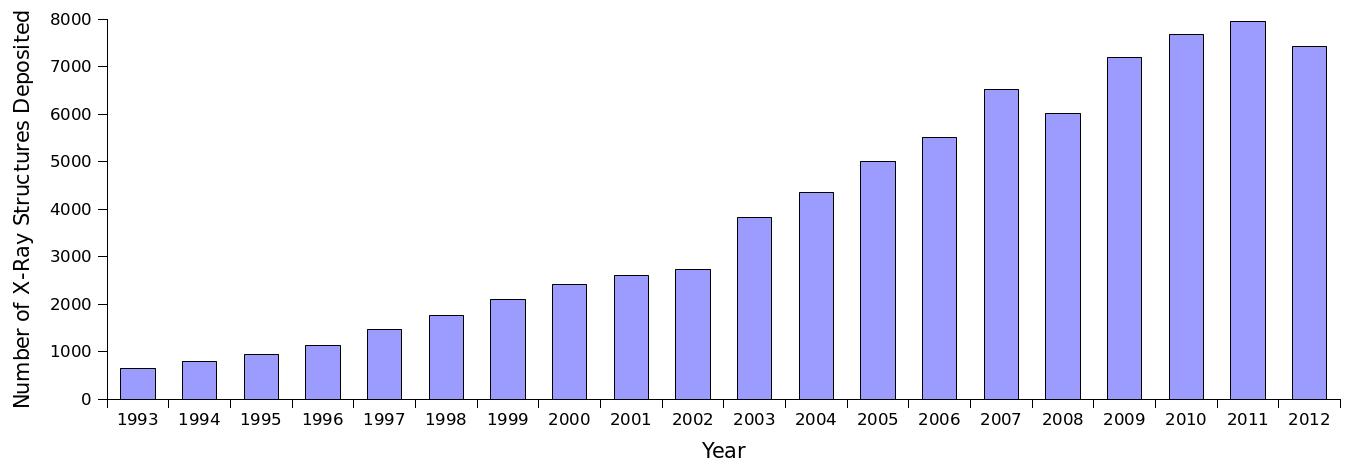
\includegraphics[width=\textwidth]{figures/pdb_deposit_rate.png}
\caption{The rate at which new structures are deposited into the PDB over the last two decades.
Due to a variety of improvements in the field of crystallography, this rate has been steadily increasing.
Plot generated using data from the PDB \protect\cite{berman2003announcing,berman2000protein}.}
\label{figure:pdb_growth}
\end{center}
\end{figure}

% expected future growth of pdb
For example, a recent advancement in the field of crystallography is ``crystal-less'' crystallography, in which small molecules are bound by a porous scaffold matrix.
The regular structure of the matrix imparts a regular packing arrangement, necessary for interpreting diffraction patterns, onto the arrangement of small molecules.
This has the potential to address one of the largest difficulties in obtaining quality structural data for proteins, which is that it is very difficult to purify and crystallize certain proteins \cite{inokuma2013x}.

% unsorted
The number of target molecules of the set of all drugs currently available on the market consists of only about five-hundred proteins.
The bottleneck in the introduction of new chemical entities is not virtual screening, but rather optimizing these hits into higher affinity leads (see \ref{subsubsection:hit_to_lead}) and eventually balancing the requirements across all characteristics to produce a new drug (see \ref{subsubsection:lead_optimization}) \cite{bleicher2003hit}.

% drug targets
Most disease implicated proteins are not targeted by current drugs and finding improved drugs for those proteins which are currently drug targets can be very difficult, and sometimes not productive. 
Therefore, new chemical entities frequently aim to target proteins that are currently not targetd by currently available drugs. 
Of the entire proteome, only \textapprox30,000 proteins are regulated by small molecule binding, making them reasonable targets of drug action.
A large number of these possible drug targets are not implicated in any disease.
Due to this and a number of other factors, estimates of the total number of the proteins regulated by small molecule binding that are possible drug targets is much lower than 30,000.
Frequently cited numbers for the number of possible drug targets in humans are six-hundred to fifteen-hundred, still significantly higher than the total number of targets exploited by current drugs \cite{imming2006drugs,overington2006many}.
Further, different families of cellular proteins are not equally likely to be targets of drugs.
As of 2002, 47\% of current drug targets are enzymes, followed by 30\% being GPCR's \cite{hopkins2002druggable}.

% drug-likeness
After identifying appropriate proteins as drug targets, focus is then turned to assessing the drug-likeness of candidate small molecules.
A number of key characteristics are generally true of drug-like small molecules:
\begin{enumerate}
\item Five or fewer hydrogen bond donors,
\item 500 Da or less total molecular mass,
\item high liphophilicity,
\item number of nitrogen and oxygen atoms is not greater than 10 \cite{rule_of_five}.
\end{enumerate}
Therefore, when screening small molecules libraries for hits, these criteria are highly prioritized.

% example of successful application of these ideas
There is an advantage to flexible substrates, which is that they can flex in order to create better contacts with the protein structure increasing binding affinity.
This is especially important as the location of heavy atoms in the target protein is frequently only known to an accuracy of ~0.4 angstroms.
Further, specific knowledge of the binding geometry between the initial lead compound and the target makes it possible to computationally screen possible chemical group substituents, to maximize binding affinity, increase solubility or bioavailability.
One of the earliest examples of the successful application of structure based drug design is the carbonic anhydrase inhibitor dorzolamide, in which most of these ideas were applied to find a drug with very high binding affinity \cite{greer1994application}.
Through understanding the protein-ligand conformation and specific contacts they were able to modify a known substrate


% limitations
Despite advantages in speed and cost due to limitations in accuracy computational screening has struggled to produce the same results as empirical screening.
However, more recently virtual screening has succeeded in producing hit rates greater than those from empirical screening techniques.
Virtual screening has been used to identified leads which were later developed into the human immunodeficiency virus (HIV) protease inhibitor Viracept, and the anti-influenza drug Relenza.
\begin{figure}[h]
    \centering
    \begin{subfigure}[b]{0.3\textwidth}
        \centering
        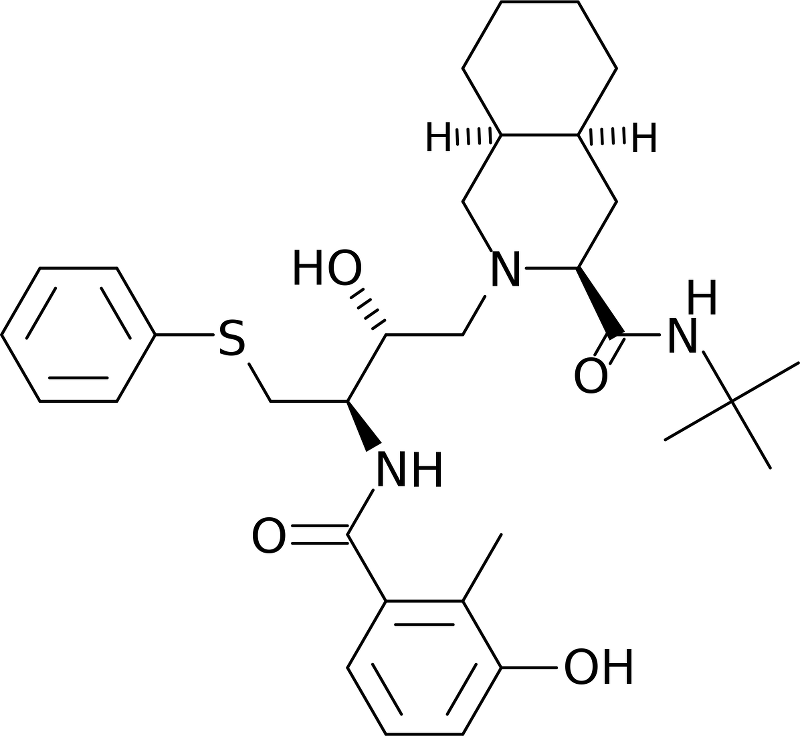
\includegraphics[width=\textwidth]{figures/nelfinavir_small.png}
        \label{fig:nelfinavir_chemical}
        \caption{}
    \end{subfigure}%
    \hspace{0.1\textwidth}
    \begin{subfigure}[b]{0.3\textwidth}
        \centering
        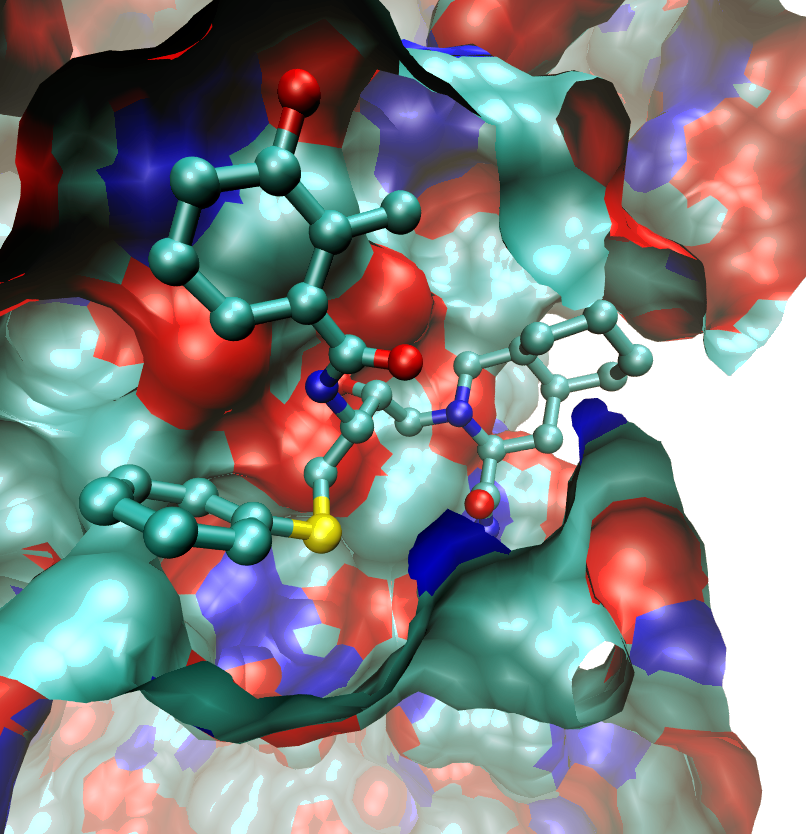
\includegraphics[width=\textwidth]{figures/complexed_nelfinavir_white.png}
        \label{fig:nelfinavir_docked}
        \caption{}
    \end{subfigure}
    \label{fig:nelfinavir}
    \caption{
The HIV protease inhibitor, nelfinavir, marketed under the name Viracept was originally identified using a computational docking screen.
It has a very high binding affinity for its target protein, 2 nM.
Here it is shown crystallized with multidrug variant (ACT) (V82T/I84V) of HIV-1 protease, PDBID 3EL5 \protect\cite{king2012extreme}.
(b) generated with Visual Molecular Dynamics \protect\cite{humphrey1996vmd} and \protect\cite{povray}.
}
\end{figure}
A number of challenges which limit the utility of docking programs have been identified
\begin{enumerate}
\item The number of possible small molecules is essentially unbounded, however only a very small fraction of these ligands are potentially drug compounds. Limiting sampling to this subspace is a challenging problem.
\item The number of conformations of ligand molecules rises exponentially with the number of internal degrees of freedom of the ligand. Sampling the huge conformational space of the ligand becomes a computationally difficult problem on its own.
\item The difficulty of accurately assessing or comparing the energy of different protein-ligand complexes or conformations\cite{shoichet2004virtual}.
\end{enumerate}

% similarity between hits and leads
It has been found that introduced drugs are often very chemically similar the hit compounds from which they were derived \cite{proudfoot2002drugs}.
So in order to increase the diversity of drugs and find drugs which are able to treat new diseases, or diseases which have evolved resistance to current drugs it may be necessary to either increase the size of the screened database or increase the possible diversity which might be increase through the hit-to-lead step.

\subsubsection{Hit-to-Lead Optimization}
\label{subsubsection:hit_to_lead}
Hit compounds generally have a binding affinity for the target protein on the order of micromolar binding.
The goals of hit-to-lead optimization are to further increase that affinity with the goal of eventually reaching binding affinities on the order of \textapprox10 nanomolar or better, find other molecules with similar chemical characteristics to increase the size and diversity of the set of lead compounds, and screen hit compounds for any obvious issues.
At this stage of computational screening, more accurate energy models are required than for the initial screen \cite{jorgensen2004many,gohlke2002approaches,jorgensen2009efficient}.

In the hit-to-lead stage, there are multiple methods used to convert hit compounds into multiple and chemically distinct lead compounds.
First, pieces of multiple hit compounds can be joined to construct larger compounds, hopefully accumulating the attractive forces of each.
Second, functional groups can be added or replaced through molecular growing and evolution techniques.
Finally, a library can be searched by chemical similarity to the initial hit compound.
In all cases, the potential lead compound is docked or grown in the known binding site of the protein target.
Docking as a means of converting hit compounds to lead compounds is very similar to docking as a means of hit generation.
However, in this case the small molecule library is restricted to chemical space surrounding hit compounds.

A popular program for building, or mutating, lead compounds is Biochemical and Organic Model Builder (BOMB) \cite{barreiro2007docking}.
BOMB can operated as either a hit identification program or as a hit-to-lead optimization method.
Working to identify new compounds, BOMB starts with a number of different small ``core'' scaffolds and attempts to increase binding affinity by adding or replacing substituents to add favorable interactions while avoiding steric clashes.
BOMB has been successfully used to evolve a hit compound that showed no inhibition of HIV reverse transcriptase (RT) into a potent non-nucleoside RT inhibitor with nanomolar level binding \cite{barreiro2007docking}.

% which is hopefully well correlated with the binding energy,
% Interestingly, it is not necessarily the case that the scoring function is anchored in a physical force field.
% It is possible to use statistical or artificial intelligence approaches with success, so long as they are able to successfully solve the classification problem of distinguishing strong binders from weak binders.
After conversion of a hit compound into a number of possible leads, a scoring function is used to rank and identify lead compounds.
This scoring function may be based either on statistical knowledge of similar structures or basic physical forces.
A successful scoring function, be it knowledge-based or physical, must be able to successfully solve the classification problem of distinguishing strong binders from weak binders.
For initial hit generation, a coarse grained energy function may be sufficient to differentiate ligands which bind strongly from those which do not bind at all.
However, in order to convert hit compounds to lead compounds, it is necessary to use a more sensitive (and generally slower) energy model to accurately rank the binding affinity of different small molecules \cite{jorgensen2004many,gohlke2002approaches}.
These energy models will be discussed in \nameref{section:energy_functions} (\ref{section:energy_functions}).

Whereas previously, lead compounds were evaluated almost exclusively on binding affinity to the target protein, recently more emphasis is being placed on identifying hit compounds that satisfy other characteristics besides binding affinity \cite{bleicher2003hit}.
It is important to begin to consider other characteristics of the potential drugs earlier in the pre-clinical process, because later it is difficult to make changes affecting characteristics such as solubility without significantly altering the binding affinity of an already highly modified hit compound.
As lead compounds are rarely very chemically distinct from the hits from which they were derived, and increasing binding affinity is actually sometimes an easier problem than addressing some of the other characteristics in the ``rule of five'', it is reasonable to begin by first trying to optimize hit compounds to satisfy some other criteria and postpone maximizing binding affinity \cite{proudfoot2002drugs}.


\subsubsection{Lead Optimization}
\label{subsubsection:lead_optimization}
In lead optimization the compounds which have been identified by the earlier steps in the process are optimized to drug molecules.
The largest differentiating factor between hit-to-lead optimization and lead optimization is the plausibility of the compound to act as a successful drug molecule.
The goals of lead optimization overlap heavily with those of the hit-to-lead stage.
Although this can include increasing binding affinity to the target even further, usually the focus is on other characteristics including selectivity, ease of synthesis, pharmacokinetic properties and intellectual property concerns \cite{keserHu2006hit}.
Computational modelling can help not only identify hit compounds, and convert those initial hits into leads, but also to help estimate absorption, distribution, metabolism, elimination, toxicology, sometimes referred to as the ADME characteristics \cite{kerns2008drug}.

Computational models for ADME characteristics ususally use regression equations or neural networks to predict these characteristics \cite{jorgensen2004many}.

Up to one half of all drugs which do not survive clinical trials, fail to do so because of lack of efficacy, which is influenced both by binding, but also by the absorption characteristics of the molecule.
The number of drugs which fail to make it through clinical trials due to toxcicity is similarly high, about 40\% \cite{li2001screening}.
Advancing a potential drug to clinical trials represents a very large financial investment, and effective computational screens of lead molecules at this point in the process can reduce the rate of failure in clinical trials, thereby having a very large impact on the final costs of new drugs brought to market.
